\documentclass[a4paper,12pt]{article}

\usepackage[utf8]{inputenc}
\usepackage[T1]{fontenc}
\usepackage[english,german]{babel}
\usepackage{fancyhdr} %Kopf und Fußzeile
\usepackage{graphicx}
\usepackage{amsmath}
\usepackage[style=authoryear]{biblatex} % BibLaTeX-Paket
\addbibresource{literatur.bib} % Pfad zur Bibliografiedatei
\graphicspath{{./bilder/}{./}}

% use last
\usepackage[colorlinks=true,allcolors=black]{hyperref}


\setlength{\parindent}{0pt} % cm, mm, in
\setlength{\parskip}{0.6ex plus 0.3ex minus 0.2ex} %elastisches Maß, um unschöne Seitenumbrüche zu vermeiden

% Kopf und Fußzeilen
\pagestyle{fancy}
\lhead{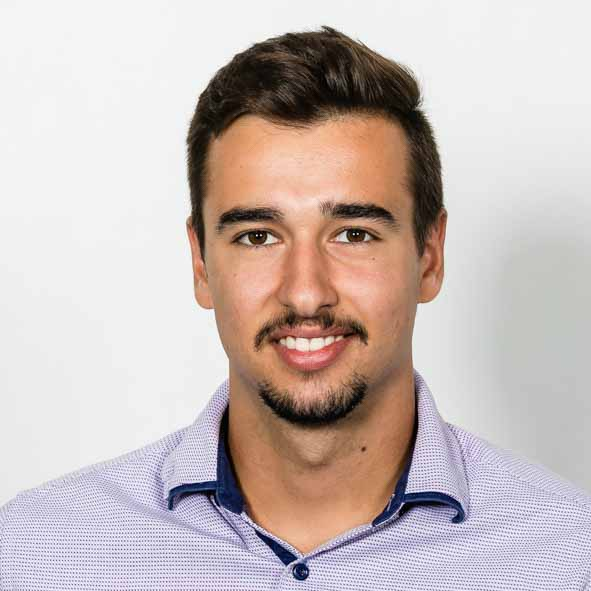
\includegraphics[height=3ex]{ASadowski}}
\rhead{\thepage}
\lfoot{2023-09-19}
\cfoot{}

\begin{document}

% !TeX root = main.tex
\begin{titlepage}

	\centering
	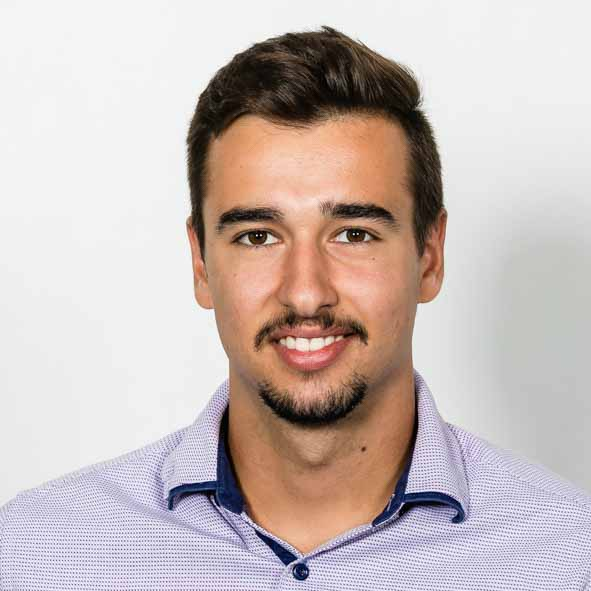
\includegraphics[width=0.15\textwidth]{ASadowski}\par\vspace{1cm}
	{\scshape\LARGE FOM - Hochschule für Oekonomie und Management \par}
	\vspace{1cm}
	{\scshape\Large Bachelor Arbeit\par}
	\vspace{1.5cm}
	{\huge\bfseries Die sehr spannende akademisch wissenschaftliche Arbeit\par}
	\vspace{2cm}
	{\Large\itshape Alexander Sadowski\par}
	\vfill
	supervised by\par
	Dr.~Mark \textsc{Brown}

	\vfill

% Bottom of the page
	{\large \today\par}
\end{titlepage}
\pagenumbering{Roman}
% !TeX root = main.tex

\section{Vorwort}

Hier steht ein Vorwort blabla 



\newpage
\tableofcontents

\newpage
\listoffigures %Abbildungsverzeichnis

\newpage
\listoftables

\newpage
% !TeX root=main.tex


\section *{Abkürzungsverzeichnis} % das Sternchen * sorgt dafür, dass die Section nicht nummeriert wird und nicht im Inhaltsverzeichnis auftaucht
\begin{description}
    \item[AI:] Artificial Intelligence
    \item[BI:] Business Intelligence
    \item[DSR:] Design Science Research
    \item[KI:] Künstliche Intelligenz
    \item[LLM:] Large Language Models
    \item[NLP:] Natural Language Processing
\end{description}


\newpage
\pagenumbering{arabic}
\thispagestyle{empty} %keine Kopf und Fußzeile oder {plain}

% !TeX root = main.tex

\section{Einleitung} 

Hello World.
Übermäßiger Likörkonsum in der Öffenltichkeit führt zu Ärger.
Übermäßiger Likörkonsum in der Öffenltichkeit führt zu Ärger.
Übermäßiger Likörkonsum in der Öffenltichkeit führt zu Ärger.
Übermäßiger Likörkonsum in der Öffenltichkeit führt zu Ärger.
Übermäßiger Likörkonsum in der Öffenltichkeit führt zu Ärger.

Gründe für die Benutzung von Computern:
\begin{itemize}
\item sie sind schnell
\item sie sind preiswert
\begin{itemize}
\item sie kosten nur wenig Steuern
\item und sind billig in der Anschaffung
\end{itemize}
\item es ist modern
\end{itemize}

\begin{enumerate}
\item suabermachen
\item überprüfen
\item reparieren
\end{enumerate}

Komponenten eines Rechners:
 \begin{description}
\item[CPU:] hier wird gerechnet
Übermäßiger Likörkonsum in der Öffenltichkeit führt zu Ärger.

\item[RAM:] das Kurzzeitgedächtnis. Übermäßiger Likörkonsum in der Öffenltichkeit führt zu Ärger.
Übermäßiger Likörkonsum in der Öffenltichkeit führt zu Ärger.

\item[DISK:] das Langzeitgedächtnis
Übermäßiger Likörkonsum in der Öffenltichkeit führt zu Ärger.
\end{description}
\subsection{Motivation}
Hello World. Der Rabatt nach\S~3 des Vertrages beträgt 2\%, das ist nicht viel und macht umgerechnet 17,45~\$, siehe Abbildung~\ref{fig:bald}
Übermäßiger Likörkonsum in der\textbf{Öffenltichkeit} führt zu Ärger. %Formtierungen
Übermäßiger Likörkonsum in der \textsl{Öffenltichkeit} führt zu Ärger.
Übermäßiger Likörkonsum in der \textit{Öffenltichkeit} führt zu Ärger.
Übermäßiger Likörkonsum\footnote{Vgl. \cite{Mitt95:Latex}} in der Öffenltichkeit führt zu Ärger.
Übermäßiger Likörkonsum in der Öffenltichkeit führt zu Ärger.

\begin{figure}[htb] %htb setzt das Bild genau and ende der subsection
\begin{center}
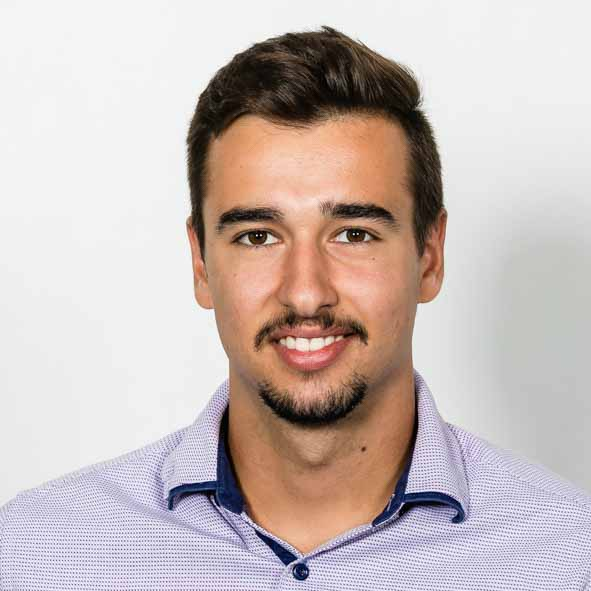
\includegraphics[scale=0.25]{ASadowski} % oder width=0.5
\end{center}

\caption{Impression von ASadowski}
\label{fig:bald}
\end{figure}

\subsection{Zielsetzung}
\label{sec:ziel} %Bezug
Hello World.
Übermäßiger Likörkonsum in der Öffenltichkeit führt zu Ärger.
Übermäßiger Likörkonsum in der Öffenltichkeit führt zu Ärger.
Übermäßiger Likörkonsum in der Öffenltichkeit führt zu Ärger.
Übermäßiger Likörkonsum in der Öffenltichkeit führt zu Ärger.
Übermäßiger Likörkonsum in der Öffenltichkeit führt zu Ärger.

Hello World.
Übermäßiger Likörkonsum in der Öffenltichkeit führt zu Ärger.
Übermäßiger Likörkonsum in der Öffenltichkeit führt zu Ärger.
Übermäßiger Likörkonsum in der Öffenltichkeit führt zu Ärger.
Übermäßiger Likörkonsum in der Öffenltichkeit führt zu Ärger.
Übermäßiger Likörkonsum in der Öffenltichkeit führt zu Ärger.


\subsection{Zielgruppe}
Hello World.
Übermäßiger Likörkonsum in der Öffenltichkeit führt zu Ärger.
Übermäßiger Likörkonsum in der Öffenltichkeit führt zu Ärger.
Übermäßiger Likörkonsum in der Öffenltichkeit führt zu Ärger.
Übermäßiger Likörkonsum in der Öffenltichkeit führt zu Ärger.
Übermäßiger Likörkonsum in der Öffenltichkeit führt zu Ärger.

\subsection{Methodik}
Hello World.
Übermäßiger Likörkonsum in der Öffenltichkeit führt zu Ärger.
Übermäßiger Likörkonsum in der Öffenltichkeit führt zu Ärger.
Übermäßiger Likörkonsum in der Öffenltichkeit führt zu Ärger.
Übermäßiger Likörkonsum in der Öffenltichkeit führt zu Ärger.
Übermäßiger Likörkonsum in der Öffenltichkeit führt zu Ärger.


% !TeX root=main.tex

\section{Grundlagen}

\subsection{Fundamentales}
Am Anfang war das Wort, siehe~\ref{sec:ziel}%es wird Bezug
. Und außerdem war es ziemlich finster\footnote{\cite{Mitt95:Latex}}.


\begin{table}[htb]
\caption{Preisliste}
\label{tab:preis}
\begin{center}
\begin{tabular}{c|l|r} % | für Linien,   mit Feldbegrenzung{c|p{60mm}|r}
Pos. & Beschreibung & Preis \\
\hline 			%Waagerechte Linie
1 & Prozessor & 198,98 \\
2 & Hauptspeicher & 87,66 \\
3 & Festplate & 128,88 \\
\hline
\multicolumn{2}{r}{Summe} & 1427,95 \\
\hline
\end{tabular}
\end{center}
\end{table}


schon Pythagoras \cite[S. 48ff]{Mitt95:Latex} wusste über das Dreieck, in der unten beschriebenen Formel~\ref{eq:wurzel}:
\begin{equation*}
a^2 + b^2 = c^2
\end{equation*}

\begin{align}
a^2 + 3\,b &=\cos \omega t \notag \\
\sqrt[3]{x^2 + y^2} &=7\,\ln \dfrac{5 + b}{7 - c} \label{eq:wurzel}
\end{align}


\begin{equation}
\left(
\begin{array}{cccc}
a_{1,1} & a_{1,2} & \cdots & a_{1,n} \\
a_{2,1} & a_{2,2} & \cdots & a_{2,n} \\
	\vdots & & \ddots & \vdots \\
a_{m,1} & a_{m,2} & \cdots & a_{m,n} \\
\end{array}
\right)
\end{equation}

\begin{align}
\sum_{i=1}^n &=n \cdot \dfrac{n+1}{2} \\
\text{e}^{\text{i}\,\pi} + 1 & = 0  % konstanten werden nicht kursiv gedruckt
\end{align}

Die Verfügbarkeit $a$ ergibt sich aus der Betriebszeit $t_{b}$ und der Geamtzeit $t_{ges}$ als
\begin{align}
availability &= \frac{operation time}{total time}  \\
&= \frac{8765 \text{h}}{8964 h} = 0,987\\
a &= \frac{t_b}{t_{ges}}
\end{align}

Sie beträgt $a = 0{,}98$ oder entsprechend 98\%. % {,} wichtig um die amerikanische Formatierung zu vermeiden

Die Fläche beträgt $A = 37$~m$^2$

\clearpage



\printbibliography 
\end{document}